\whiteBGstarBegin
\setcounter{section}{0}
\section{Lý thuyết: Hiện tượng phóng xạ hạt nhân và các loại tia phóng xạ}
\begin{enumerate}[label=\bfseries Câu \arabic*:]
	\item \mkstar{1} [1]
	
	\cauhoi
	{Phóng xạ hạt nhân là phản ứng ...
		\begin{mcq}(2)
			\item nhiệt hạch.
			\item hạt nhân thu năng lượng.
			\item phân hạch.
			\item hạt nhân tỏa năng lượng.
		\end{mcq}
	}
	
	\loigiai
	{		\textbf{Đáp án: D.}
		
		Phóng xạ hạt nhân là phản ứng hạt nhân tỏa năng lượng.
		
	}
	
	\item \mkstar{1} [1]
	
	\cauhoi
	{Phản ứng hạt nhân nào sau đây là quá trình phóng xạ?
		\begin{mcq}(2)
			\item $\ce{^210_84 Po} \longrightarrow \ce{^4_2 He} + \ce{^206_82 Pb}$.
			\item $\ce{^1_0 n} + \ce{^235_92 U} \longrightarrow \ce{^139_54 Xe} + \ce{^95_38 Sr} + 2 \ce{^1_0 n}$.
			\item $\ce{^7_3 Li} + \ce{^2_1 H} \longrightarrow 2 \ce{^4_2 He} + \ce{^1_0 n}$.
			\item $\ce{^4_2 He} + \ce{^27_13 Al} \longrightarrow \ce{^1_0 n} + \ce{^30_15 P}$.
		\end{mcq}
	}
	
	\loigiai
	{		\textbf{Đáp án: A.}
		
		Phản ứng
		$$\ce{^210_84 Po} \longrightarrow \ce{^4_2 He} + \ce{^206_82 Pb}$$
		là quá trình phóng xạ.
		
		Các phản ứng còn lại là phản ứng nhiệt hạch, phân hạch hoặc phản ứng hạt nhân thông thường.
		
	}
		\item \mkstar{1} [3]
	
	\cauhoi
	{Chọn phát biểu đúng về tia phóng xạ $\alpha$.
		\begin{mcq}
			\item Không bị lệch khi đi qua điện trường và từ trường.
			\item Có vận tốc bằng vận tốc ánh sáng trong chân không.
			\item Là dòng các hạt nhân $\ce{^4_2 He}$.
			\item Có khả năng đâm xuyên mạnh hơn tia phóng xạ $\gamma$.
		\end{mcq}
	}
	
	\loigiai
	{		\textbf{Đáp án: C.}
		
		Tia phóng xạ $\alpha$ là dòng các hạt nhân $\ce{^4_2 He}$, có bị lệch trong điện trường và từ trường, khả năng đâm xuyên yếu hơn và vận tốc nhỏ hơn nhiều so với tia $\gamma$.
		
	}
	
	\item \mkstar{1} [3]
	
	\cauhoi
	{Tia nào sau đây \textbf{không} phải là tia phóng xạ?
		\begin{mcq}(4)
			\item Tia $\alpha$.
			\item Tia $\beta^+$.
			\item Tia $\gamma$.
			\item Tia X.
		\end{mcq}
	}
	
	\loigiai
	{		\textbf{Đáp án: D.}
		
		Tia X bản chất là sóng điện từ, không phải tia phóng xạ.
		
	}
	\item \mkstar{1} [12]
	
	\cauhoi
	{Cặp tia nào dưới đây có cùng bản chất là sóng điện từ?
		\begin{mcq}(2)
			\item Tia $\beta ^+$ và tia $\alpha$.
			\item Tia hồng ngoại và tia tử ngoại.
			\item Tia $\alpha$ và tia tử ngoại.
			\item Tia $\beta ^+$ và tia $\beta ^-$.
		\end{mcq}
	}
	
	\loigiai
	{		\textbf{Đáp án: B.}
		
		Tia hồng ngoại và tia tử ngoại đều có bản chất là sóng điện từ.
		
	}
	\item \mkstar{1} [5]

\cauhoi
{Hạt nhân $\ce{^A_Z X}$ phóng xạ $\alpha$ tạo ra hạt nhân $\ce{Y}$. Phương trình phản ứng có dạng:
	\begin{mcq}(2)
		\item $\ce{^A_Z X} \longrightarrow \alpha + \ce{^{A-4}_{Z-2} Y}$.
		\item $\ce{^A_Z X} \longrightarrow \alpha + \ce{^{A-2}_{Z-4} Y}$.
		\item $\ce{^A_Z X} \longrightarrow \alpha + \ce{^{A-2}_{Z-2} Y}$.
		\item $\ce{^A_Z X} \longrightarrow \alpha + \ce{^{A-4}_{Z-4} Y}$.
	\end{mcq}
}

\loigiai
{		\textbf{Đáp án: A.}
	
	Áp dụng định luật bảo toàn số khối và bảo toàn điện tích thì phản ứng đúng là
	$$\ce{^A_Z X} \longrightarrow \alpha + \ce{^{A-4}_{Z-2} Y}$$
	
}
\item \mkstar{1} [5]

\cauhoi
{Hạt nhân $\ce{^A_Z X}$ phóng xạ $\beta^-$ tạo ra hạt nhân $\ce{Y}$. Phương trình phản ứng có dạng:
	\begin{mcq}(2)
		\item $\ce{^A_Z X} \longrightarrow \beta^- + \ce{^{A}_{Z-1} Y}$.
		\item $\ce{^A_Z X} \longrightarrow \beta^- + \ce{^{A-1}_{Z} Y}$.
		\item $\ce{^A_Z X} \longrightarrow \beta^- + \ce{^{A+1}_{Z} Y}$.
		\item $\ce{^A_Z X} \longrightarrow \beta^- + \ce{^{A}_{Z+1} Y}$.
	\end{mcq}
}

\loigiai
{		\textbf{Đáp án: D.}
	
	Áp dụng định luật bảo toàn số khối và bảo toàn điện tích thì phản ứng đúng là
	$$\ce{^A_Z X} \longrightarrow \beta^- + \ce{^{A}_{Z+1} Y}$$
	
}
	\item \mkstar{2} [1]
	
	\cauhoi
	{Đồng vị $\ce{^30_15 P}$ biến thành hạt nhân $\ce{^30_14 Si}$ sau khi phóng xạ tia
		\begin{mcq}(4)
			\item $\beta^-$. 
			\item $\gamma$. 
			\item $\beta^+$. 
			\item $\alpha$. 
		\end{mcq}
	}
	
	\loigiai
	{		\textbf{Đáp án: C.}
		
		Phương trình phản ứng:
		$$\ce{^30_15 P} \longrightarrow \ce{^30_14 Si} + \ce{^A_Z X}$$
		
		Áp dụng định luật bảo toàn số khối và bảo toàn điện tích, tìm được X là hạt $\beta^+$ ($\ce{^0_1 e}$).
		
	}
	

	\item \mkstar{2} [13]

\cauhoi
{Hạt nhân $\ce{^226_88 Ra}$ phóng xạ ra 3 hạt $\alpha$ và một hạt $\beta^-$ trong chuỗi phóng xạ liên tiếp. Khi đó hạt nhân tạo thành là
	\begin{mcq}(4)
		\item $\ce{^214_82 X}$.
		\item $\ce{^212_83 X}$.
		\item $\ce{^214_83 X}$.
		\item $\ce{^212_82 X}$.
	\end{mcq}
}

\loigiai
{		\textbf{Đáp án: C.}
	
	Phương trình phản ứng:
	$$\ce{^226_88 Ra}\ \ldots \longrightarrow \ldots\ 3 \ce{^4_2 He} + \ce{^0_{-1} e} + \ce{X}$$
	
	Áp dụng định luật bảo toàn số khối và bảo toàn điện tích, tìm được $X$ là $\ce{^214_83 X}$.
	
}
	\item \mkstar{2} [5]

\cauhoi
{Khi một hạt nhân nguyên tử phóng xạ lần lượt một tia $\alpha$ rồi một tia $\beta^+$ thì hạt nhân nguyên tử sẽ biến đổi như thế nào?
	\begin{mcq}
		\item Số khối giảm 4, số neutron giảm 1.
		\item Số neutron giảm 3, số proton giảm 1.
		\item Số proton giảm 1, số neutron tăng 3.
		\item Số khối giảm 4, số proton tăng 1.
	\end{mcq}
}

\loigiai
{		\textbf{Đáp án: A.}
	
	Phương trình phản ứng:
	$$\ce{^A_Z X}\ \ldots \longrightarrow \ldots\ \ce{^4_2 He} + \ce{^0_1 e} + Y$$
	
	Áp dụng định luật bảo toàn số khối và bảo toàn điện tích, tìm được Y là $\ce{^{A-4}_{Z-3} Y}$.
	
	Vậy số khối giảm 4, số proton giảm 3, dẫn đến số neutron giảm 1.
	
}

\end{enumerate}

\loigiai
{
	\begin{center}
		\textbf{BẢNG ĐÁP ÁN}
	\end{center}
	\begin{center}
		\begin{tabular}{|m{2.8em}|m{2.8em}|m{2.8em}|m{2.8em}|m{2.8em}|m{2.8em}|m{2.8em}|m{2.8em}|m{2.8em}|m{2.8em}|}
			\hline
			1.D  & 2.A  & 3.C  & 4.D  & 5.B  & 6.A  & 7.D & 8.C & 9.C & 10.A \\
			\hline
			
		\end{tabular}
	\end{center}
}

\section{Dạng bài: Định luật phóng xạ}
\begin{enumerate}[label=\bfseries Câu \arabic*:]
		\item \mkstar{1} [1]
	
	\cauhoi
	{Một chất phóng xạ có chu kì bán rã $T=\SI{8}{h}$, hằng số phân rã của chất phóng xạ này bằng
		\begin{mcq}(4)
			\item $\SI{1.2e-5}{s^{-1}}$.
			\item $\SI{2.4e-5}{s^{-1}}$.
			\item $\SI{2.6e-5}{s^{-1}}$.
			\item $\SI{1.3e-5}{s^{-1}}$.
		\end{mcq}
	}
	
	\loigiai
	{		\textbf{Đáp án: B.}
		
		Hằng số phân rã:
		$$\lambda = \dfrac{\ln 2}{T} = \dfrac{\ln 2}{\SI{28800}{s}} = \SI{2.4e-5}{s^{-1}}$$
		
	}
	\item \mkstar{1} [5]
	
	\cauhoi
	{Hằng số phóng xạ của Rubidi là $\SI{0.00077}{s^{-1}}$. Chu kì bán rã của nó tính theo đơn vị phút nhận giá trị nào sau đây?
		\begin{mcq}(4)
			\item 150 phút.
			\item 15 phút.
			\item 900 phút.
			\item 600 phút.
		\end{mcq}
	}
	
	\loigiai
	{		\textbf{Đáp án: B.}
		
		Hằng số phóng xạ được tính theo công thức:
		$$\lambda = \dfrac{\ln 2}{T} \Rightarrow T = \SI{900}{s}$$
		
		Vậy $T=15$ phút.
		
	}

		\item \mkstar{2} [13]
	
	\cauhoi
	{Ban đầu có $\SI{4e20}{}$ hạt nhân $\ce{^60_27 Co}$ với chu kì bán rã là $T=\SI{5.3}{}$ năm. Số hạt nhân $\ce{^60_27 Co}$ còn lại sau 10,6 năm bằng
		\begin{mcq}(4)
			\item $\SI{0.5e20}{}$.
			\item $\SI{2e20}{}$.
			\item $\SI{1e20}{}$.
			\item $\SI{0.2e20}{}$.
		\end{mcq}
	}
	
	\loigiai
	{		\textbf{Đáp án: C.}
		
		Số hạt nhân còn lại:
		$$N=N_0 2^{-\frac{t}{T}} = \SI{1e20}{}$$
		
	}
	\item \mkstar{2} [13]
	
	\cauhoi
	{Chất phóng xạ iốt $\ce{^131_53 I}$ có chu kì bán rã là $T=8$ ngày đêm. Ban đầu có $\SI{16e19}{}$ hạt nhân chất này. Sau 24 ngày đêm, số hạt nhân $\ce{^131_53 I}$ bị phân rã bằng
		\begin{mcq}(4)
			\item $\SI{4.8e20}{}$.
			\item $\SI{2e19}{}$.
			\item $\SI{5.3e19}{}$.
			\item $\SI{1.4e20}{}$.
		\end{mcq}
	}
	
	\loigiai
	{		\textbf{Đáp án: D.}
		
		Số hạt nhân bị phân rã:
		$$\Delta N = N_0 (1-2^{-\frac{t}{T}}) = \SI{1.4e20}{}$$
		
	}
\item \mkstar{2} [5]

\cauhoi
{Một lượng chất phóng xạ có khối lượng ban đầu $m_0$. Sau 4 chu kì bán rã khối lượng chất phóng xạ còn lại là
	\begin{mcq}(4)
		\item $\dfrac{m_0}{5}$.
		\item $\dfrac{m_0}{25}$.
		\item $\dfrac{m_0}{16}$.
		\item $\dfrac{m_0}{50}$.
	\end{mcq}
}

\loigiai
{		\textbf{Đáp án: C.}
	
	Sau 4 chu kì bán rã $(t=4T)$ thì khối lượng chất phóng xạ còn lại là:
	$$m=m_0 2^{-\frac{t}{T}} = m_0 \cdot \dfrac{1}{16}$$
	
	Vậy $m=\dfrac{m_0}{16}$.
	
}
	\item \mkstar{3} [1]
	
	\cauhoi
	{Hạt nhân Pôlôni $(\ce{^210_84 Po})$ phóng ra hạt $\alpha$ và biến thành hạt nhân Chì $(\ce{Pb})$ bền, có chu kì bán rã là 138 ngày. Ban đầu có một mẫu Pôlôni nguyên chất có khối lượng $\SI{30}{g}$. Cho số A-vô-ga-đrô $N_\text{A} = \SI{6.02e23}{mol^{-1}}$. Sau 414 ngày số hạt nhân Chì hình thành bằng
		\begin{mcq}(4)
			\item $\SI{7.671e22}{}$.
			\item $\SI{7.525e23}{}$.
			\item $\SI{7.671e23}{}$.
			\item $\SI{7.525e22}{}$.
		\end{mcq}
	}
	
	\loigiai
	{		\textbf{Đáp án: D.}
		
		Số hạt Pôlôni ban đầu:
		$$N_0 = \dfrac{m}{M} N_\text{A} = \SI{8.6e22}{}$$
		
		Số hạt Chì tạo thành cũng đồng thời là số hạt Pôlôni bị phân rã:
		$$\Delta N=N_0 (1-2 ^{-\frac{t}{T}} )= \SI{7.525e22}{}$$
		
	}
	
	\item \mkstar{3} [1]
	
	\cauhoi
	{I-ốt $(\ce{^131_53 I})$ là chất phóng xạ $\beta^-$ với chu kì bán rã 8 ngày. Ban đầu có $\SI{200}{g}$ I-ốt $(\ce{^131_53 I})$. Khối lượng I-ốt trên bị phân rã trong ngày thứ 10 kể từ thời điểm ban đầu là
		\begin{mcq}(4)
			\item $\SI{115.9}{g}$.
			\item $\SI{8.39}{g}$.
			\item $\SI{7.61}{g}$.
			\item $\SI{84}{g}$.
		\end{mcq}
	}
	
	\loigiai
	{		\textbf{Đáp án: C.}
		
		Khối lượng I-ốt trên bị phân rã trong ngày thứ 10 là hiệu giữa khối lượng bị phân rã cuối ngày 10 với cuối ngày 9 kể từ thời điểm ban đầu.
		
		Khối lượng I-ốt bị phân rã cuối ngày 10:
		$$\Delta N_1 = N_0 (1-2^{-\frac{t_1}{T}}) = \SI{115.9}{g}$$
		
		Khối lượng I-ốt bị phân rã cuối ngày 9:
		$$\Delta N_2 = N_0 (1-2^{-\frac{t_2}{T}}) = \SI{108.3}{g}$$
		
		Vậy khối lượng I-ốt trên bị phân rã trong ngày thứ 10 là $\Delta N_1 - \Delta N_2 = \SI{7.6}{g}$.
		
	}
	
	\item \mkstar{3} [3]
	
	\cauhoi
	{Chất phóng xạ $\ce{X}$ có chu kì bán rã là $\SI{8.5}{s}$. Ban đầu có một mẫu $\ce{X}$ nguyên chất. Sau bao lâu thì số hạt nhân $\ce{X}$ bị phân rã bằng 15 lần số hạt nhân $\ce{X}$ còn lại trong mẫu?
		\begin{mcq}(4)
			\item $\SI{38.0}{s}$.
			\item $\SI{8.5}{s}$.
			\item $\SI{34.0}{s}$.
			\item $\SI{25.5}{s}$.
		\end{mcq}
	}
	
	\loigiai
	{		\textbf{Đáp án: C.}
		
		Số hạt bị phân rã bằng 15 lần số hạt còn lại:
		$$\dfrac{\Delta N}{N} = 15 \Rightarrow \dfrac{1-2^{-\frac{t}{T}}}{2^{-\frac{t}{T}}} = 15 \Rightarrow t = \SI{34.0}{s}$$
		
	}
	\item \mkstar{3} [13]
	
	\cauhoi
	{
		Chất phóng xạ X có số hạt nhân giảm dần theo thời gian như đồ thị. Chu kì bán rã của chất phóng xạ X bằng
		\begin{mcq}(2)
			\item 16 ngày đêm.
			\item 10 ngày đêm.
			\item 6 ngày đêm.
			\item 8 ngày đêm.
		\end{mcq}
		\begin{center}
			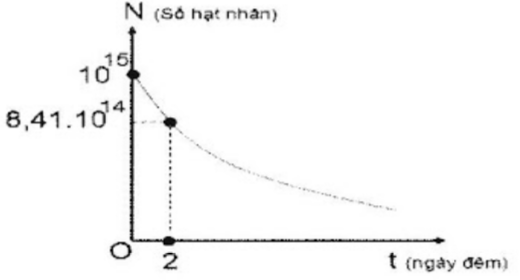
\includegraphics[scale=0.8]{../figs/VN12-2021-PH-TP038-1}
		\end{center}
		
	}
	
	\loigiai
	{		\textbf{Đáp án: D.}
		
		Tại thời điểm $t=0$ thì $N_0 = \SI{e15}{}$.
		
		Tại thời điểm $t=2$ thì $N=\SI{8.41e14}{}$.
		
		Áp dụng công thức:
		$$N=N_0 2^{-\frac{t}{T}} \Rightarrow T = 8$$
		
	}
	\item \mkstar{4} [10]
	
	\cauhoi
	{Ban đầu $(t=0)$ có một mẫu chất phóng xạ X nguyên chất. Ở thời điểm $t$ số hạt nhân X chưa bị phân rã bằng $20\%$ số hạt nhân ban đầu. Đến thời điểm $t+100\ \text{s}$ số hạt nhân X chưa bị phân rã bằng $5\%$ số hạt nhân ban đầu. Chu kì bán rã của chất phóng xạ đó là
		\begin{mcq}(4)
			\item 50 s.
			\item 25 s.
			\item 400 s. 
			\item 200 s.
		\end{mcq}
	}
	
	\loigiai
	{		\textbf{Đáp án: A.}
		
		Ở thời điểm $t$ số hạt nhân X chưa bị phân rã bằng $20\%$ số hạt nhân ban đầu:
		
		$$\dfrac{N}{N_0}=\dfrac{1}{5} \Rightarrow 2^{-\frac{t}{T}} = \dfrac{1}{5}$$
		
		Đến thời điểm $t+100\ \text{s}$ số hạt nhân X chưa bị phân rã bằng $5\%$ số hạt nhân ban đầu:
		
		$$\dfrac{N}{N_0}=\dfrac{1}{20} \Rightarrow 2^{-\frac{(t+100)}{T}} = \dfrac{1}{20} \Rightarrow 2^{-\frac{t}{T}} \cdot 2^{-\frac{-100}{T}} = \dfrac{1}{20} \Rightarrow T = \SI{50}{s}$$
	}


\item \mkstar{4} [13]

\cauhoi
{Ban đầu có $N_0$ hạt nhân của chất phóng xạ X có chu kì bán rã là $T$, gọi $\Delta t$ là khoảng thời gian mà số hạt nhân còn lại của một lượng chất phóng xạ giảm đi $e$ lần so với ban đầu (với $\ln e = 1$). Nếu sau khoảng thời gian $\SI{0.5}{} \Delta t$ số hạt nhân chất phóng xạ X còn lại bằng bao nhiêu phần trăm so với lúc ban đầu?
	\begin{mcq}(4)
		\item $\SI{70.71}{\percent}$. 
		\item $\SI{50.00}{\percent}$.
		\item $\SI{60.65}{\percent}$.
		\item $\SI{82.44}{\percent}$.
	\end{mcq}
}

\loigiai
{		\textbf{Đáp án: C.}
	
	Dựa vào công thức $N=N_0 e^{-\lambda \Delta t}$, để $N$ giảm đi $e$ lần so với ban đầu thì $\dfrac{N}{N_0} = \dfrac{1}{e} = e^{-1}$. Do đó:
	$$-\lambda \Delta t = -1 \Rightarrow \Delta t = \dfrac{1}{\lambda}$$
	
	Sau khoảng thời gian $\SI{0.5}{} \Delta t$ thì số hạt còn lại là
	$$\dfrac{N}{N_0} = e^{-\lambda \cdot \frac{1}{2\lambda}} = \SI{60.65}{\percent}$$
	
}


\end{enumerate}

\loigiai
{
	\begin{center}
		\textbf{BẢNG ĐÁP ÁN}
	\end{center}
	\begin{center}
		\begin{tabular}{|m{2.8em}|m{2.8em}|m{2.8em}|m{2.8em}|m{2.8em}|m{2.8em}|m{2.8em}|m{2.8em}|m{2.8em}|m{2.8em}|}
			\hline
			1.B  & 2.B  & 3.C  & 4.D  & 5.C  & 6.D  & 7.C & 8.C & 9.D & 10.A \\
			\hline
			11.C  & & & & & & & & &  \\
			\hline
			
		\end{tabular}
	\end{center}
}


\whiteBGstarEnd